\documentclass[border=4pt]{standalone}
\usepackage[compat=1.1.0]{tikz-feynman}
\usepackage{amsmath}

\begin{document}
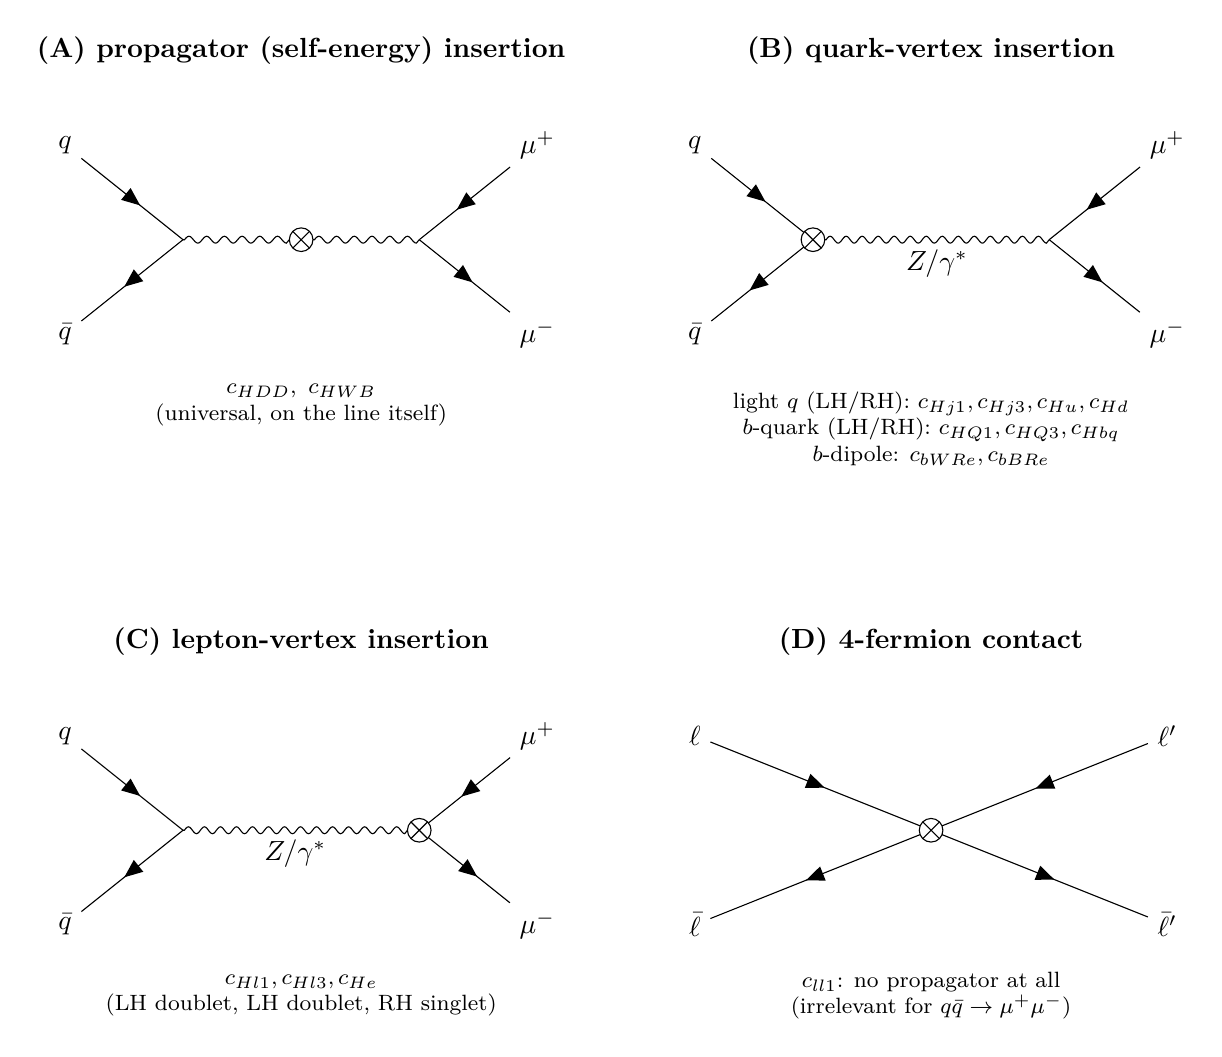
\begin{tikzpicture}

% ---------- (A) self-energy insertion: cHDD, cHWB ----------
\begin{scope}[shift={(0,0)}]
  \node at (3,2.4) {\textbf{(A) propagator (self-energy) insertion}};
  \begin{feynman}
    \vertex (q) at (0,1.2) {\(q\)};
    \vertex (qbar) at (0,-1.2) {\(\bar{q}\)};
    \vertex (a) at (1.5,0);
    \vertex[crossed dot] (op) at (3,0) {};
    \vertex (b) at (4.5,0);
    \vertex (mup) at (6,1.2) {\(\mu^{+}\)};
    \vertex (mum) at (6,-1.2) {\(\mu^{-}\)};
    \diagram* {
      (q) -- [fermion] (a) -- [fermion] (qbar),
      (a) -- [boson] (op) -- [boson] (b),
      (mup) -- [fermion] (b) -- [fermion] (mum),
    };
  \end{feynman}
  \node[align=center, font=\footnotesize] at (3,-2.1) {\(c_{HDD},\ c_{HWB}\) \\ (universal, on the line itself)};
\end{scope}

% ---------- (B) quark-side vertex insertion ----------
\begin{scope}[shift={(8,0)}]
  \node at (3,2.4) {\textbf{(B) quark-vertex insertion}};
  \begin{feynman}
    \vertex (q) at (0,1.2) {\(q\)};
    \vertex (qbar) at (0,-1.2) {\(\bar{q}\)};
    \vertex[crossed dot] (a) at (1.5,0) {};
    \vertex (b) at (4.5,0);
    \vertex (mup) at (6,1.2) {\(\mu^{+}\)};
    \vertex (mum) at (6,-1.2) {\(\mu^{-}\)};
    \diagram* {
      (q) -- [fermion] (a) -- [fermion] (qbar),
      (a) -- [boson, edge label'=\(Z/\gamma^{*}\)] (b),
      (mup) -- [fermion] (b) -- [fermion] (mum),
    };
  \end{feynman}
  \node[align=center, font=\footnotesize] at (3,-2.4) {light \(q\) (LH/RH): \(c_{Hj1},c_{Hj3},c_{Hu},c_{Hd}\) \\ \(b\)-quark (LH/RH): \(c_{HQ1},c_{HQ3},c_{Hbq}\) \\ \(b\)-dipole: \(c_{bWRe},c_{bBRe}\)};
\end{scope}

% ---------- (C) lepton-side vertex insertion ----------
\begin{scope}[shift={(0,-7.5)}]
  \node at (3,2.4) {\textbf{(C) lepton-vertex insertion}};
  \begin{feynman}
    \vertex (q) at (0,1.2) {\(q\)};
    \vertex (qbar) at (0,-1.2) {\(\bar{q}\)};
    \vertex (a) at (1.5,0);
    \vertex[crossed dot] (b) at (4.5,0) {};
    \vertex (mup) at (6,1.2) {\(\mu^{+}\)};
    \vertex (mum) at (6,-1.2) {\(\mu^{-}\)};
    \diagram* {
      (q) -- [fermion] (a) -- [fermion] (qbar),
      (a) -- [boson, edge label'=\(Z/\gamma^{*}\)] (b),
      (mup) -- [fermion] (b) -- [fermion] (mum),
    };
  \end{feynman}
  \node[align=center, font=\footnotesize] at (3,-2.1) {\(c_{Hl1},c_{Hl3},c_{He}\) \\ (LH doublet, LH doublet, RH singlet)};
\end{scope}

% ---------- (D) 4-fermion contact: cll1 ----------
\begin{scope}[shift={(8,-7.5)}]
  \node at (3,2.4) {\textbf{(D) 4-fermion contact}};
  \begin{feynman}
    \vertex (l1) at (0,1.2) {\(\ell\)};
    \vertex (l1bar) at (0,-1.2) {\(\bar{\ell}\)};
    \vertex[crossed dot] (c) at (3,0) {};
    \vertex (l2) at (6,1.2) {\(\ell'\)};
    \vertex (l2bar) at (6,-1.2) {\(\bar{\ell}'\)};
    \diagram* {
      (l1) -- [fermion] (c) -- [fermion] (l1bar),
      (l2) -- [fermion] (c) -- [fermion] (l2bar),
    };
  \end{feynman}
  \node[align=center, font=\footnotesize] at (3,-2.1) {\(c_{ll1}\): no propagator at all \\ (irrelevant for \(q\bar q \to \mu^+\mu^-\))};
\end{scope}

\end{tikzpicture}
\end{document}
